%
%  outline latex source document for AILP assignment 3.
%  use pdflatex to format this (and bibtex if use external bibliography)
%
\documentclass[10pt,a4paper]{article}
\usepackage[a4paper,hmargin=1.25in,vmargin=1in]{geometry}
\usepackage{amssymb,amsmath}            % if some maths is needed
\usepackage{graphicx}                   % if any images are to be included
% pick a different font if desired
\usepackage{times}
\usepackage{subfigure}
\usepackage{caption}
\usepackage{enumerate}
\usepackage{graphicx}
\usepackage{cite}
\usepackage{url}
\usepackage{algorithm}  
\usepackage{algorithmicx}  
\usepackage{algpseudocode}  
\usepackage{amsmath}  
\usepackage{amssymb} 
\usepackage{listings}  

\setlength{\parindent}{0cm}
\setlength{\parskip}{4pt}

\floatname{algorithm}{Algorithm}  
\renewcommand{\algorithmicrequire}{\textbf{Input:}}  
\renewcommand{\algorithmicensure}{\textbf{Output:}} 
\def\UrlBreaks{\do\A\do\B\do\C\do\D\do\E\do\F\do\G\do\H\do\I\do\J\do\K\do\L\do\M\do\N\do\O\do\P\do\Q\do\R\do\S\do\T\do\U\do\V\do\W\do\X\do\Y\do\Z\do\[\do\\\do\]\do\^\do\_\do\`\do\a\do\b\do\c\do\d\do\e\do\f\do\g\do\h\do\i\do\j\do\k\do\l\do\m\do\n\do\o\do\p\do\q\do\r\do\s\do\t\do\u\do\v\do\w\do\x\do\y\do\z\do\.\do\@\do\\\do\/\do\!\do\_\do\|\do\;\do\>\do\]\do\)\do\,\do\?\do\'\do+\do\=\do\#}  
\usepackage{appendix}
%% Define a new 'leo' style for the package that will use a smaller font.
\makeatletter
\def\url@leostyle{%
	\@ifundefined{selectfont}{\def\UrlFont{\sf}}{\def\UrlFont{\small\ttfamily}}}
\makeatother
%% Now actually use the newly defined style.
\urlstyle{leo}


\title{Advanced Vision Practical
 (2018) Report}               % AILP: please use this title.
\author{Yu, Jianmeng \quad Yi, Ruitao }                      % replace with name or exam number
\date{\today}                 % replace with actual date

\begin{document}

\maketitle  % this inserts title, author info
%
\section{Introduction}
The task is to construct a complete box form 50 3D point clouds acquired by a Kinect sensor. One can get a complete box if all the 3D points captured in each frame could be processed and transformed into points in the initial frame. 

\section{Algorithms and implementation}
\subsection{Extract the relevant data from each point cloud}  
\subsubsection{Description}
The key idea for data extraction is how to construct a mask to eliminate the irrelevant data. First, we need to erase the data points that are distant from the box we concerned. 
Then, the following two type of irrelevant data are removed: 
\begin{itemize}
   \setlength{\parskip}{-1pt}
	\item \textbf{Background Blue Data Points} - using {\tt removeBlue.m}, to remove these data points coming from the lab window.
	\item \textbf{Skin-coloured Data Points} -  using {\tt removeBlue.m}, to remove the detection on the hand holding the box.
\end{itemize} 
During the faraway data eliminating process, we only retain data which is within a interval of \emph{[Center $\pm$ Offset]}, where the center is provided by the material and the offset is estimated by our group. 
%The colorspace and minimum/maximum values for each channel of the colorspace were set in the App,
This process result in a binary mask of size 424x512, marking the area of valid box points.
Also, the technique of Erode and Dilate is used to remove noise points found at edge of the box.
Occasionally, this process will fail to filter some hand data points.
However, these points are filtered out at the plane extraction stage of the project.

Using this binary mask, the project could use the extracted points to construct a new Point Cloud, filtering out the irrelevant data points.
Result of this process on point cloud is shown in Fig \ref{fig:21} and Fig \ref{fig:22}.
And the effect on original image is shown in Fig \ref{fig:23} and Fig \ref{fig:24}.



\subsubsection{Algorithm}

The Pseudo-code of the algorithm is shown in Algorithm \ref{alg:mask}. 
The original Matlab code is in Appendix \ref{algapp:mask}.



     \begin{algorithm}  
	\caption{Relevant data extraction} 
     \label{alg:mask} 
	\begin{algorithmic}[1]  
		\Require $Frame\; number$ 
		\Ensure $Extracted\; point\; cloud$  
		\Function {GetPointCloud}{$frameNum$}  
		\State $Colour \gets \;$\Call{GetColour}{$frameNum$}
		\State $Location \gets \;$\Call{GetLocation}{$frameNum$}
		\State $Mask \gets \;$\Call{GetMask}{$frameNum$}
		\State $Count \gets 1$
		\For {$i= \;1: maxRow$}  
		\For {$j= \;1: maxColumn$} 
		\If {$valid \; point(i,j,:) \;\&\& \;mask(i,j,:)\ne0 $}
		\State $RGB\{Count\} = Colour(i,j,:)$
		\State $XYZ\{Count\} = Location(i,j,:)$
		\EndIf
		\EndFor
		\EndFor
		\State $results \gets \;Point \;cloud \;reconstructed \;using \;RGB \;and \;XYZ$
		\State \Return{$result$}  
		\EndFunction  
		%\State  
		\Function{GetColour}{$frameNum$}
		\State $Colour \gets \; pc\{frameNum\}.Colour $  
		\State $results\gets flip(rot90(reshape(Colour,{\rm{ }}[\max Row,{\rm{ }}\max Column,{\rm{ }}3])))$  
		\State \Return{$result$}  
        \EndFunction  
		%\State  
        \Function{GetLocation}{$frameNum$}
        \State $Location \gets \; pc\{frameNum\}.Location $  
        \State $results\gets flip(rot90(reshape(Location,{\rm{ }}[\max Row,{\rm{ }}\max Column,{\rm{ }}3])))$  
        \State \Return{$result$}  
        \EndFunction  
 		%\State  
        \Function{GetMask}{$frameNum$}
        \State $Center \gets {\rm{[ - 0}}{\rm{.71, - 0}}{\rm{.30, 0}}{\rm{.81]}} $  
        \State $Offset \gets {\rm{[ - 0}}{\rm{.15, 0}}{\rm{.20, 0}}{\rm{.25]}}$  
        \State ${\rm{Mask1  \gets  }}\left\{ \begin{array}{l}
        1{\rm{\; if \; Location}} \in {\rm{[Center - Offset\;,\;Center + Offset]}}\\
        0{\rm{\; otherwise}}
        \end{array} \right.$  
        \State $Mask2  \gets removeSkin \{$\Call{GetColour}{$frameNum$}$\} $
        \State $Mask3  \gets removeBackground \{$\Call{GetColour}{$frameNum$}$\} $
        \State $results\gets denoise(Mask1)\; \&\& \;denoise(Mask2)\; \&\& \; denoise(Mask3)$        
        \State \Return{$result$}  
        \EndFunction        

	\end{algorithmic}  
\end{algorithm}  


\vspace{-10pt}
\hspace{-40pt}
\begin{figure}[!h]
\hspace{-50pt}
\begin{minipage}[t]{0.74 \linewidth}
	
	\centering
	\includegraphics[width=.5\textwidth]{p2}
	\captionsetup{font={small}}
	\caption{ \small Raw data from frame 19}
    \label{fig:21}
\end{minipage}
\hspace{-100pt}
\begin{minipage}[t]{0.74 \linewidth}
	\centering
	\includegraphics[width=.5\textwidth]{p1}
	\captionsetup{font={small}}
	\caption{ \small Extract the relevant data from frame 19}
    \label{fig:22}
\end{minipage}
\end{figure}

\vspace{-10pt}
\hspace{-40pt}
\begin{figure}[!h]
\hspace{-50pt}
\begin{minipage}[t]{0.74 \linewidth}
	
	\centering
	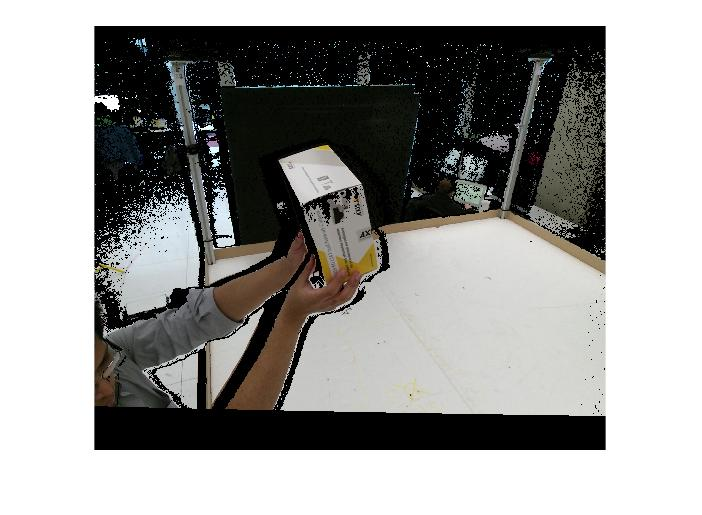
\includegraphics[scale=0.3]{unmasked.jpg}
	\captionsetup{font={small}}
	\caption{ \small Raw Image from Frame 36}
    \label{fig:23}
\end{minipage}
\hspace{-100pt}
\begin{minipage}[t]{0.74 \linewidth}
	\centering
	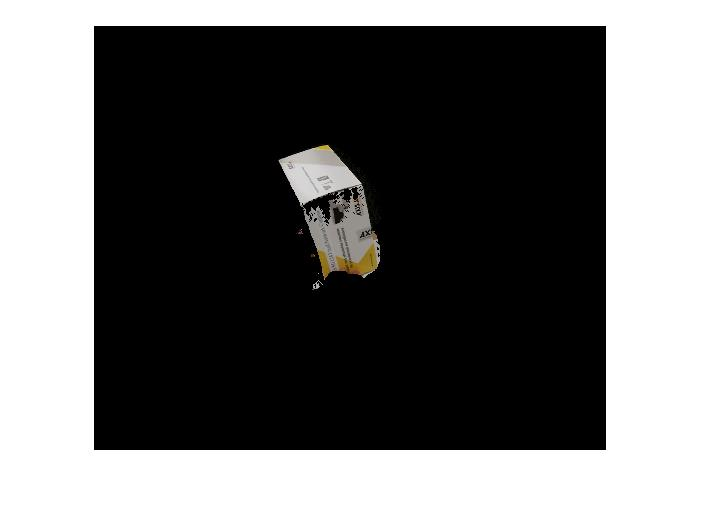
\includegraphics[scale=0.3]{masked.jpg}
	\captionsetup{font={small}}
	\caption{ \small Masked Image from Frame 36}
    \label{fig:24}
\end{minipage}
\end{figure}


%\subsubsection{Performance}

\newpage

\subsection{Extract the planes from each point cloud}  
\subsubsection{Description}
The main idea of this step is that we extract raw planes with the supplied "Patch-growth" algorithm.
And by doing it multiple times, we filter out the misfit planes and obtain a clean set of plane. 
\begin{enumerate}[1.]
	\item Raw plane extraction \\
First, we define the maximum number of planes we want per frame. 
Then, for each iteration, we select a patch from the remaining points, and generate a plane with the patch. 
After that, for each point left, we add it to the patch if the distance to this patch plane is smaller than the tolerance.
Once the loop is complete enough points, we remove the points from the list, and store the plane normal. 
	
	\item Get cleaned plane \\
The key idea in this part is that how to de-noise the plane got from the first stage and how to re-mark the intersection points lying on the intersecting planes. 
Firstly, for each round, we get the raw planes and sort them by the number of points on it in descending order. 
The plane with the maximum number of points is selected. 
For each remaining possible planes, we average the planes within 15 degree angle of the selected plane.
And we drop all other plane within 60 degrees angle (We assumed the box surface are orthogonal to each other).
Finally, for all cleaned planes, we first remove intersection points from their originally marked planes and then we assign them to the plane with minimum distance. 

\end{enumerate}


%\subsubsection{Algorithm}
The Pseudo-code of the algorithm is shown in Algorithm \ref{alg:plane}. 
The original Matlab code is in Appendix \ref{algapp:plane}.

%\subsubsection{Performance}
And the result of this process on point cloud is shown in Fig \ref{fig:31} and Fig \ref{fig:32}.

\vspace{-10pt}
\hspace{-40pt}
\begin{figure}[!h]
	\hspace{-50pt}
	\begin{minipage}[t]{0.74 \linewidth}
		
		\centering
		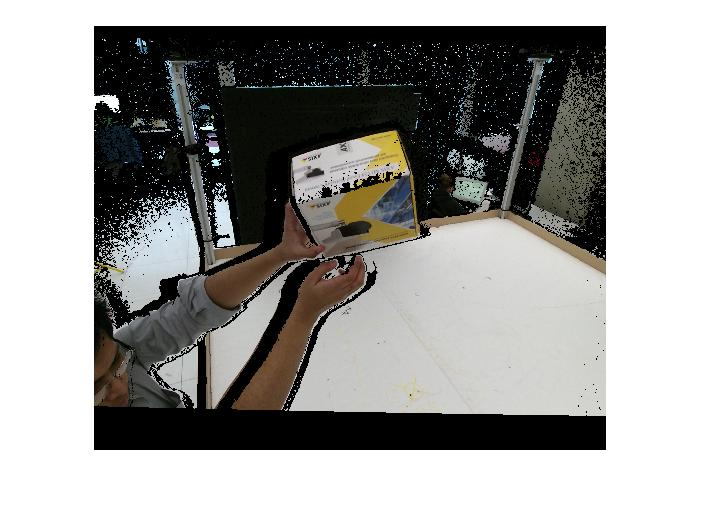
\includegraphics[scale=0.3]{planeandnormalori.jpg}
		\captionsetup{font={small}}
		\caption{ \small Raw data from frame 6}
		\label{fig:31}
	\end{minipage}
	\hspace{-100pt}
	\begin{minipage}[t]{0.74 \linewidth}
		\centering
		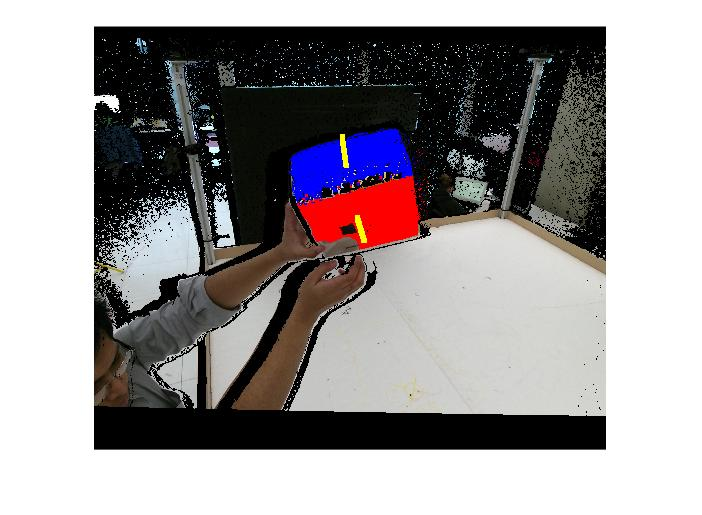
\includegraphics[scale=0.3]{planeandnormal.jpg}
		\captionsetup{font={small}}
		\caption{ \small Extract the planes from frame 6}
		\label{fig:32}
	\end{minipage}
\end{figure}

\begin{algorithm}  
	\caption{Clean planes extraction} 
	\label{alg:plane} 
	\begin{algorithmic}[1]  
		\Require $Frame\; number, \; Plot(boolean, optional)$ 
		\Ensure $Planesout:(a,b,c,d){\rm{\; which\; corresponds \;to\; }}ax + by + cz + d = 0 \qquad \qquad$
		\Ensure $ Pointsout: \;points \;on \;each \;plane$  
		\Function {getCleanPlane}{$frameNum,plot$}  
		\State $Location \gets$ \Call{GetPC}{$frameNum$}$.Location$
		\State $Planes \gets \emptyset$
		\State $Points \gets \emptyset$
		\For {$each \; round$}  
		\State $[Tempplane, Temppoint] \gets$ \Call{GetPlanes}{$Location$}
		\State $Planes \gets Catenate(Planes,Tempplane)$
        \State $Points \gets Catenate(Points,Histogram \;of \;Temppoint)$		
		\EndFor
		\For {$each \;iteration$}
		\State $Sort \;the \;Planes \;by \;the \;number \;of\; Points \;assigned \;to \;it \;in \;descending \;order$
		\State $MaxPlane \gets Planes\{1\}$
        \For {$i = 1: num \;of \;remaining \;Planes$}  
        \State $Normal1 \gets MaxPlane(1:3)$ 
        \State $Normal2 \gets Plane\{i\}(1:3)$ 
        \State $Angle \gets arccos(Normal1,Normal2)$	
        \If { $angle <= $MAXANG }
        $Mark\; Plane\{i\} \;as\; candidate\; plane$
        \ElsIf { MAXANG $< angle <= $REJANG }
        $Remove\; Plane\{i\}$
        \EndIf	
        \EndFor	
        \State $NewPlane \gets Average \;all\;candidate \;planes$
        \State $PossiblePlaneNum \gets PossiblePlaneNum + 1$
        \EndFor
        \For {$all \;Possible \;Planes$}
        \State $Store \;points \;on \;intersection \;lines$
        \State $Remove \;intersection \;points \;from \;their \;originally \;marked \;plane$
        \EndFor	
        \For {$each \;intersection\;point$}
        \State $Re-assign \;it \;to \;the\;plane \;with \;minimum \;orthogonal \;distance$
        \EndFor
		\State $results\gets updated\; possible \;planes$         
		\State \Return{$result$}  
		\EndFunction  
		
		
		\State  
		\Function{GetPlanes}{$Location$}
		\State $Remaining  \gets Location $  
		\For {$i = 1:MaxIteration$}
		\State $[Plane\{i\}, remaining] \gets Select\_Patch\{remaining\}$  
		\For {$each \;remaining \; point$}
		\State $measure \;distance \;from \;this \;point \;to \;Plane \{i\}$
		\If {$distance < threshold$}
		\State $Add \;this \;point \;to \;Plane \{i\}$
		\EndIf
		\EndFor
		\EndFor
		\State $results\gets [Plane, points]$
		\State \Return{$result$}  
		
		\EndFunction  

		
	\end{algorithmic}  
\end{algorithm}  


\newpage

\subsection{Estimate the 3D positions of the corners where planes meet}  
\subsubsection{Description}
There could be a maximum of 3 cleaned planes for each frame. 
If a frame have less than 2 planes, there should be no corners, so we ignore frames. 
The algorithm has two core steps:
\begin{itemize}
	\item Obtain reasonable points on the intersection lines
	
	To get reasonable data points, first, we need to calculate the unit vector pointing to the direction of the intersection line of two intersecting planes. Then, we project all the points on the vector and select all data points between quantiles 0.04 and 0.96 before winsorizing all reasonable data points.
	\item Forming a corner 
	
    If there are two planes in this frame, then for each plane, we project all points of this plane in the direction of the normal of another plane. After that, we select the furthest projected point as a new corner point which should lie on the edge of that plane. If there are three planes, assume that we have done the first step with plane1 and plane2. For each pair (Plane1, Plane3) and (Plane2, Plane3), first, we project all points of this plane on the direction of the normal of the remaining plane and select the furthest projected point as a new corner point which should lie on the edge of that plane afterwards. 
\end{itemize}


The Pseudo-code of the algorithm is shown in Algorithm \ref{alg:corner}. 
The original Matlab code is in Appendix \ref{algapp:corner}.

%\subsubsection{Performance}
And the result of this process on point cloud is shown in Fig \ref{fig:41} and Fig \ref{fig:42}.

\vspace{-10pt}
\hspace{-40pt}
\begin{figure}[!h]
	%\hspace{-50pt}
	\begin{minipage}[t]{0.3 \linewidth}
		
		\centering
		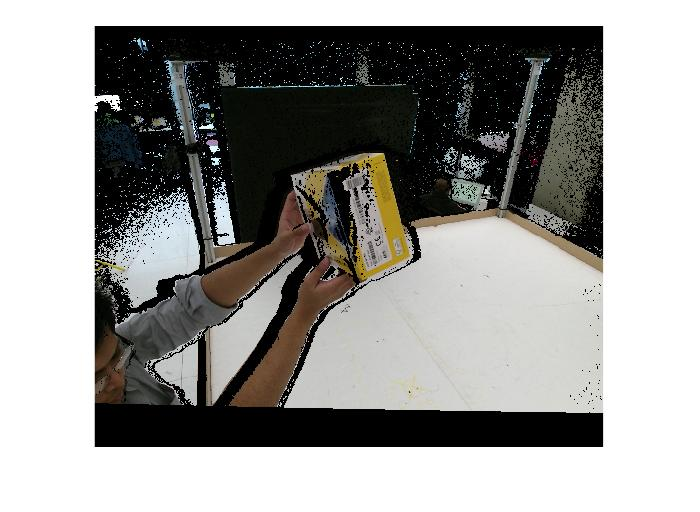
\includegraphics[scale=0.2]{cornerori.jpg}
		\captionsetup{font={small}}
		\caption{ \small Raw data from frame 19}
		\label{fig:41}
	\end{minipage}
	\begin{minipage}[t]{0.74 \linewidth}
	%\hspace{-100pt}
		\centering
		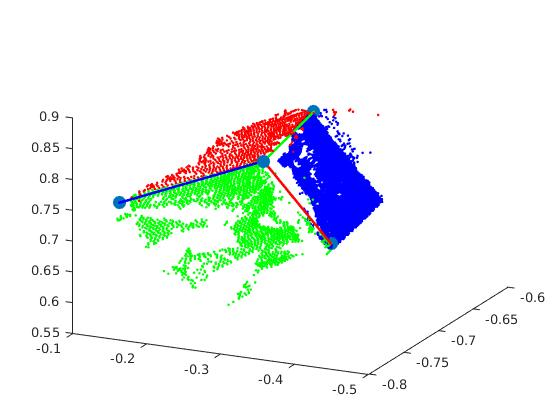
\includegraphics[scale=0.5]{corner.jpg}
		\captionsetup{font={small}}
		\caption{ \small Extracted corners from frame 19}
		\label{fig:42}
	\end{minipage}
\end{figure}


%\subsubsection{Algorithm}
\begin{algorithm}  
	\caption{Corners 3D estimation} 
	\label{alg:corner} 
	\begin{algorithmic}[1]  
		\Require $Planes, Points(get from GETCLEANPLANE)$ 
		\Ensure $Corners$
		\Function {getCorner}{$arg1, planes, points$}  
		\State $NPS \gets Num \;of \;Clean \;Planes \;extracted$
		
		
		\If { $NPS == 1$ }
		\State $Corners \gets \emptyset$
		\ElsIf { $NPS == 2$ }
		\State $[Points\_12, Vector\_12] \gets $\Call {getPlaneIntersection}{Planes\{1\}, Planes\{2\}}
		\State $Tps \gets project \; all \; points \; on \;Vector\_12$
        \State $Reasonable \;points \gets$ \Call {prctile}{Tps,[lowerbound,upperbound]}
        \State $Winsorize \;Tps $
        \State $Corners\{1\} \gets Nearest \;reasonable \;point$
        \State $Corners\{2\} \gets Furthest \; reasonable\; point$		
        \State $Corners\{3\} \gets$\Call{addAnotherPoint}{$Normal1,Plane2,Corners\{1\}$}    
        \State $Corners\{4\} \gets$\Call{addAnotherPoint}{$Normal2,Plane1,Corners\{1\}$}                
		\ElsIf { $NPS == 3$ }
		\State $[Points\_12, Vector\_12] \gets $\Call {getPlaneIntersection}{Planes\{1\}, Planes\{2\}}
		\State $Tps \gets project \; all \; points \; on \;Vector\_12$
		\State $Reasonable \;points \gets$ \Call {prctile}{Tps,[lowerbound,upperbound]} 
		\State $Intersection \;point \gets $\Call {getPlaneLineIntersection}{$Planes\{3\}, Points\_12, Vector\_12$}
		\State $Shift\; Reasonable \;points \; in \; the \;direction\;of\;the \; Intersection\;Points $
		\State $Winsorize \;Tps $		
        \State $Corners\{1\} \gets Nearest \;reasonable \;point$
        \State $Corners\{2\} \gets Furthest \; reasonable\; point$
        \State $Corners\{3\} \gets $\Call{getanotherIntersection}{$Normal1,Planes\{2\},Planes\{3\}, NP$}
        \State $Corners\{4\} \gets $\Call{getanotherIntersection}{$Normal2,Planes\{1\},Planes\{3\}, NP$}        
		\EndIf	
		\State $results\gets Corners$         
		\State \Return{$result$}  
		\EndFunction  
		
		
		\State  
		\Function{addAnotherPoint}{$Normal, Plane, Startpoint$}
		\State $Points \gets Project \;all \;points \;on \;Plane\; to \;Normal $  
		\If {$Mean(Points) < 0$}
		\State $Corner \gets Points \;assigned \;with \;Negative \;Largest \;Value$
		\Else
		\State $Corner \gets Points \;assigned \;with \;Largest \;Value$
		\EndIf
		\State $results\gets Corner$         
		\State \Return{$result$}  
		\EndFunction 
		
		\State  
		\Function{getanotherIntersection}{$Normal, Plane1, Plane2, Startpoints$}
		
	    \State $Points \gets Project \;all \;points \;on \;Plane1 \;and \;Plane2 \;to \;Normal $  
		\If {$Mean(Points) < 0$}
		\State $Corner \gets Points \;assigned \;with \;Negative \;Largest \;Value$
		\Else
		\State $Corner \gets Points \;assigned \;with \;Largest \;Value$
		\EndIf
		\State $results\gets Corner$         
		\State \Return{$result$}  
		\EndFunction 
		
	\end{algorithmic}  
\end{algorithm} 

\newpage

\subsection{Corners and point clouds normalization }  
\subsubsection{Description}
%
In order to fuse the images to the same system, we need to translate the planes onto XY, XZ, YZ planes for easier fusion.
This is possible due to the 3D object we are fusing is a box.

To do the normalization, we need to estimate the rotation and translation separately. 
For the translation part, we shift the point cloud and the corner in each frame, in order to make the axis point of corner extracted from the previous stage locating at the origin of the new reference frame. For the rotation step, we need to make sure the three axes of the corner coinciding with the positive X, Y, and Z axis respectively. 

To do this, we estimate the first rotation matrix by rotating the first axis so that it coincides with the positive X-axis, then the second rotation matrix is estimated by rotating the third axis so that coinciding with the positive Y-axis. Aggregate rotation matrix is estimated by multiplying the first and second rotation matrix. 

After this rotation, we project all marked points onto their corresponding plane, forming a smooth plane surface.

The Pseudo-code of the algorithm is shown in Algorithm \ref{alg:rotate}. 
The original Matlab code is in Appendix \ref{algapp:rotate}.

%\subsubsection{Performance}
And the result of this process on point cloud is shown in Fig \ref{fig:51}.

%\subsubsection{Algorithm}

\begin{algorithm}  
	\caption{Corners and point clouds normalization} 
	\label{alg:rotate}  
	\begin{algorithmic}[1]  
		\Require $Frame \;Number$ 
		\Ensure $Location: points mapped to plane$
		\Ensure $Corners: swapped corners$
		\Ensure $newPoints: new marked points (removing points outside the box)$
		\Function {getRotatedPoints}{$frameNum$}  
		\State $[Planes, Points] \gets$ \Call{getCleanPlane}{$frameNum$}
		\State $Corners \gets Translate($ \Call{getCorner}{$frameNum, Planes, Points$}$)$
		\State $Location \gets Translate(pc.Location)$
		\State $X \gets [1,0,0]$
		\State $Y \gets [0,1,0]$
		\State $Z \gets [0,0,1]$
		
		\State $\% \;First,select \;a \;corner\;vector \;and \;make \;it\; coincide \;with \;the \;X $
		\State $project\_XY \gets Project \;Corners{2} \;on \;XY \;plane $
		\State $rotation1 \gets$\Call{RotateZ}{Angle(projection\_XY, X)}
		\State $rotation2 \gets$\Call{RotateY}{Angle(rotation1 * Corners\{2\}, X)}
		\State $\% \;Then,select \;another \;corner\;vector \;and \;make \;it\; coincide \;with \;the \;Y $
		\State $rotation3 \gets$\Call{RotateX}{Angle(rotation1 * rotation2 * Corners\{4\}, Y)}
		\State $\% \;Finally,the \;aggregate
		 \;rotation \; matrix$	
		\State $rotation \gets rotation1 * rotation2 * rotation3$
		\For {$i = 1: number of points$}
		\State $Remark \;points\{i\}$
		\State $Points \gets$ \Call{projectPointOnLine}{Location\{i\},[0 0 0],Corners\{PN\}}
		\State $Location\{i\} \gets rotation * Location\{i\} - Points$
		\State $Corners \gets rotation * Corners;$
		\State $result\gets [Location,Corners,Points]$         
		\State \Return{$result$}  
		\EndFor
		\EndFunction
		
	\end{algorithmic}  
\end{algorithm}  

\vspace{-10pt}
\hspace{-40pt}
\begin{figure}[!h]
	%\hspace{-100pt}
		\centering
		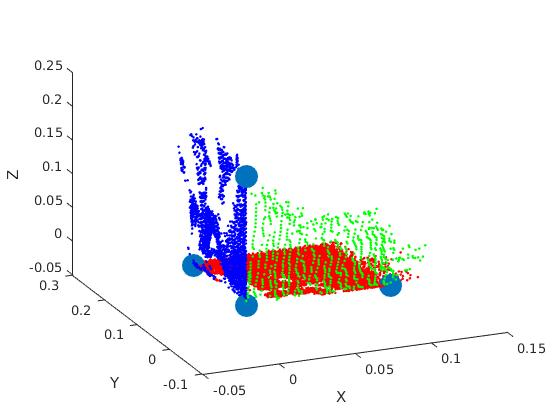
\includegraphics[scale=0.5]{rotated.jpg}
		\captionsetup{font={small}}
		\caption{ \small Frame 19 corners, rotated onto the main axis system.}
		\label{fig:51}
\end{figure} 


\newpage

\subsection{Rotation and Translation Estimation and Box Fusion}
\subsubsection{Description}
To make sure we have corner points and vectors matched correctly between two consecutive frames, we do this manually by marking the change to the red plane and the position of the blue plane in each frame. 
Then, giving the reference frame transformation from the previous stage, we map all of the points from the frame (other than 1,2,3,50 because we do not get any planes from these frames) to frame 4. Finally, we reconstruct the point clouds consecutively to fuse the whole box. 

\subsubsection{Marking System}
This project uses manual marking for plane matching due to the similarity between planes, and the most of the plane points on original point cloud image is absent.

The provided {\tt model.m} script is executed when Matlab starts, it sets several global variables used in plane extraction and model fusion.
The description of detailed marking method are in the comment section of Appendix \ref{app:model}.

\subsubsection{Algorithm}
\label{sec:thatonewithfinalimage}

Algorithm \ref{alg:fuse} shows the Pseudo-code of this step. Figures of the step-by-step fusion is included in Section \ref{sec:evaluation}. The Fig \ref{fig:6} shows the final fused model.

\vspace{-10pt}
\hspace{-40pt}
\begin{figure}[!h]
	%\hspace{-100pt}
		\centering
		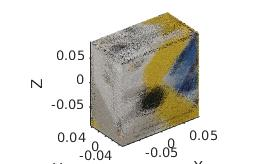
\includegraphics[scale=0.5]{box/49.jpg}
		\captionsetup{font={small}}
		\caption{ \small Final fused box}
		\label{fig:6}
\end{figure} 


\begin{algorithm}[!h]
	\caption{Rotation and Translation Estimation and Box Fusion}  
	\label{alg:fuse}
	\begin{algorithmic}[1]  
		\Require $-$
		\Ensure $Point Clouds$
		\Function {fuseModel}{}  
		\State $estimated\_size \gets [0.1700,0.090,0.1700]$
		\State $\% To \;make \;the\;box \;face \;you $
		\State $rotation \gets RotateX(270) * RotateZ(180)$
		\State $\%Calculate\; the \;center\;of\;the\;box $
		\State $Center \gets - (estimated\_size / 2)$
		\For {$i = 1: MaxFrameNum$}
		\State $pc \gets getPC(i)$
		\State $[planes,\sim] \gets$ \Call{getCleanPlane}{i}
		\State $[location, \sim, points] \gets$ \Call{getRotatedPoints}{i}
		\State $Colour \gets pc.Colour$
		\State $\% Consider\;the\;red\;plane$
		\If {$Change \;to \;the\;red\;plane$}
		\If {$Change \;to \;top$}
		\State $rotation \gets rotation * RotateX(90)$
		\ElsIf {$Change \;to \;right$}
		\State $rotation \gets rotation * RotateY(90)$
		\ElsIf {$Change \;to \;bottom$}
		\State $rotation \gets rotation * RotateX(270)$
		\ElsIf {$Change \;to \;left$}
        \State $rotation \gets rotation * RotateY(270)$
		\EndIf	
		\EndIf
		
		\State
		\State $\% Consider\;the\;blue\;plane$
		\If {$Blue \;plane\;exists$}
		\If {$on\;top$}
		\State $rotation2 \gets rotation * RotateZ(270)$
		\ElsIf {$on \;right$}
		\State $rotation2 \gets rotation * RotateZ(0)$
		\ElsIf {$on \;bottom$}
        \State $rotation2 \gets rotation * RotateZ(90)$	
		\ElsIf {$on \;left$}
        \State $rotation2 \gets rotation * RotateZ(90)$			
		\EndIf
		\EndIf
		
		\State
		\If {$Only\; one \;plane \;in \;this \;frame$}
		\State $Continue$
		\EndIf
		\State
		\For {$j = 1: number \;of \;points$}
		\State $\% Rotate \;back \;to \;original \;box$
		\State $Location(j) \gets rotation2 * Location(j)$
		\State $this\_Center \gets Center .* sign(rotation2*[1;1;1])$
		\State $\% Translation$
		\State $Location(j) \gets Location + this\_Center$
		\EndFor
		
		\State $Remove \;data \;points \;outside \;the \;box$
		
		\State $Reconstruct \;the \;point \;clouds$
		
		\EndFor 
		\EndFunction
	
	\end{algorithmic}  
\end{algorithm}  

\newpage

\section{Model evaluation}
\label{sec:evaluation}

\subsection{Images of Fused Point Clouds}
\label{sec:lotsofimage}

The following images shows the fusing of the model at different stages of the fusing. Note that there are a total of 33 frames used for the fusing of the final model show in Figure \ref{fig:6} in Section \ref{sec:thatonewithfinalimage}.

The following frames are used in the fusion of the model, the later ones are not plotted due to similarity:

 4,5,6,9,11,12,13,15,16,17,18,19,20,21,22,24,26,27,28,30,31,33,34,35,36,39,40,42,43,44,46,47,49.

\vspace{-10pt}
\hspace{-40pt}
\begin{figure}[!h]
	%\hspace{-50pt}
	\begin{minipage}[t]{0.33 \linewidth}
		
		\centering
		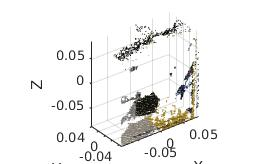
\includegraphics[scale=0.5]{box/4.jpg}
		\captionsetup{font={small}}
		\caption{ \small Frame 4}
	\end{minipage}
	\begin{minipage}[t]{0.33 \linewidth}
	%\hspace{-100pt}
		\centering
		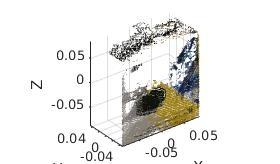
\includegraphics[scale=0.5]{box/5.jpg}
		\captionsetup{font={small}}
		\caption{ \small Frame 5}
	\end{minipage}
	\begin{minipage}[t]{0.33 \linewidth}
	%\hspace{-100pt}
		\centering
		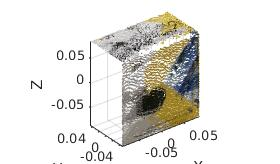
\includegraphics[scale=0.5]{box/6.jpg}
		\captionsetup{font={small}}
		\caption{ \small Frame 6}
	\end{minipage}
\end{figure}

\vspace{-30pt}
\hspace{-40pt}
\begin{figure}[!h]
	%\hspace{-50pt}
	\begin{minipage}[t]{0.33 \linewidth}
		
		\centering
		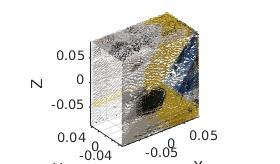
\includegraphics[scale=0.5]{box/9.jpg}
		\captionsetup{font={small}}
		\caption{ \small Frame 9}
	\end{minipage}
	\begin{minipage}[t]{0.33 \linewidth}
	%\hspace{-100pt}
		\centering
		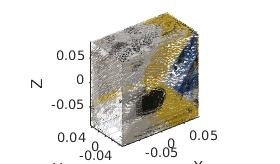
\includegraphics[scale=0.5]{box/11.jpg}
		\captionsetup{font={small}}
		\caption{ \small Frame 11}
	\end{minipage}
	\begin{minipage}[t]{0.33 \linewidth}
	%\hspace{-100pt}
		\centering
		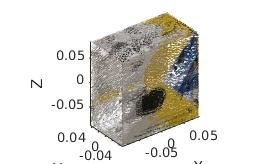
\includegraphics[scale=0.5]{box/12.jpg}
		\captionsetup{font={small}}
		\caption{ \small Frame 12}
	\end{minipage}
\end{figure}

\vspace{-30pt}
\hspace{-40pt}
\begin{figure}[!h]
	%\hspace{-50pt}
	\begin{minipage}[t]{0.33 \linewidth}
		
		\centering
		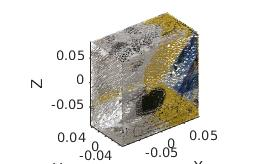
\includegraphics[scale=0.5]{box/13.jpg}
		\captionsetup{font={small}}
		\caption{ \small Frame 13}
	\end{minipage}
	\begin{minipage}[t]{0.33 \linewidth}
	%\hspace{-100pt}
		\centering
		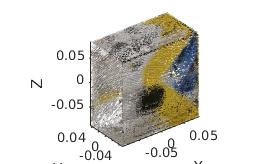
\includegraphics[scale=0.5]{box/15.jpg}
		\captionsetup{font={small}}
		\caption{ \small Frame 15}
	\end{minipage}
	\begin{minipage}[t]{0.33 \linewidth}
	%\hspace{-100pt}
		\centering
		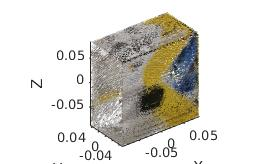
\includegraphics[scale=0.5]{box/16.jpg}
		\captionsetup{font={small}}
		\caption{ \small Frame 16}
	\end{minipage}
\end{figure}


\vspace{-30pt}
\hspace{-40pt}
\begin{figure}[!h]
	%\hspace{-50pt}
	\begin{minipage}[t]{0.33 \linewidth}
		
		\centering
		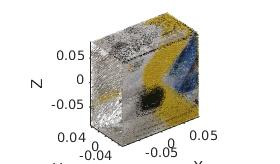
\includegraphics[scale=0.5]{box/18.jpg}
		\captionsetup{font={small}}
		\caption{ \small Frame 18}
	\end{minipage}
	\begin{minipage}[t]{0.33 \linewidth}
	%\hspace{-100pt}
		\centering
		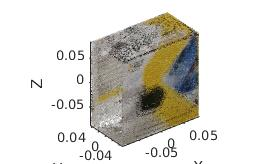
\includegraphics[scale=0.5]{box/22.jpg}
		\captionsetup{font={small}}
		\caption{ \small Frame 22}
	\end{minipage}
	\begin{minipage}[t]{0.33 \linewidth}
	%\hspace{-100pt}
		\centering
		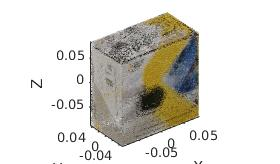
\includegraphics[scale=0.5]{box/24.jpg}
		\captionsetup{font={small}}
		\caption{ \small Frame 24}
	\end{minipage}
\end{figure}
\vspace{-20pt}
\hspace{-40pt}
\begin{figure}[!h]
	%\hspace{-50pt}
	\begin{minipage}[t]{0.33 \linewidth}
		
		\centering
		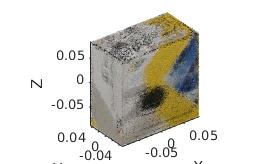
\includegraphics[scale=0.5]{box/28.jpg}
		\captionsetup{font={small}}
		\caption{ \small Frame 28}
	\end{minipage}
	\begin{minipage}[t]{0.33 \linewidth}
	%\hspace{-100pt}
		\centering
		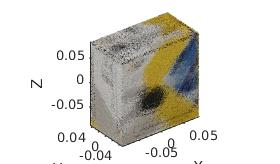
\includegraphics[scale=0.5]{box/36.jpg}
		\captionsetup{font={small}}
		\caption{ \small Frame 36}
	\end{minipage}
	\begin{minipage}[t]{0.33 \linewidth}
	%\hspace{-100pt}
		\centering
		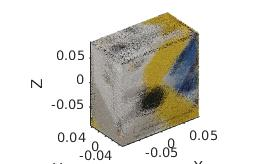
\includegraphics[scale=0.5]{box/40.jpg}
		\captionsetup{font={small}}
		\caption{ \small Frame 40}
	\end{minipage}
\end{figure}

\newpage


\subsection{Large Plane Fusion Errors}

Due to the assumption on the box shape, the plane normals obtained are orthogonal to each other.
This change has led to a drastic decrease in the fused planes.

From the figures above in Section \ref{sec:lotsofimage}, the large planes are strictly fixed onto each faces of the box. 
This change have led to almost no angular error and corner error.

The only possible error from the plane fusion can come from the transformation in {\tt getRotatePoints}. 
In this section, the points are projected onto the XYZ coordinate system.
However, due to the erraticity caused during recording of the frames, the planes all have an angle of intersection greater than 90.
This intersection angle may lead to the shrinking or rotation error on the extracted planes.
The following Figure shows such error, note that the error is barely noticeable when comparing the images. 

The blurry planes in the final image are caused by this effect, even in the case when large error has occured, the frame could be removed easily by modifying {\tt model.m} file.

Fig \ref{fig:e1} and Fig \ref{fig:e2} shows the difference caused by the error.
Note the shadow added at top of the plane, the increase in brightness, and the image is slightly shifted upward.

\vspace{-10pt}
\hspace{-40pt}
\begin{figure}[!h]
	%\hspace{-50pt}
	\begin{minipage}[t]{0.5 \linewidth}
		
		\centering
		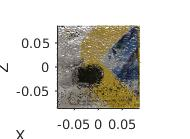
\includegraphics[scale=0.5]{planeerror13.jpg}
		\captionsetup{font={small}}
		\caption{ \small Fused Box at frame 13}
		\label{fig:e1}
	\end{minipage}
	\begin{minipage}[t]{0.5 \linewidth}
	%\hspace{-100pt}
		\centering
		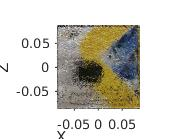
\includegraphics[scale=0.5]{planeerror15.jpg}
		\captionsetup{font={small}}
		\caption{ \small Fused Box at frame 15}
		\label{fig:e2}
	\end{minipage}
\end{figure}

\subsection{Angular and Corner Position Error}

Due to the assumption of box shape, such errors are eliminated during the fusion of the box.
Hence the cumulative error required could not be plotted.
Corner Positions are fixed by the model.m, so no position error could be made in the project.

Instead, this project will plot a chart of the angular error eliminated during each step. 

Figure \ref{fig:e3} shows the (average) angular error in each frame.
Red bar shows the average error between 3 planes are used, blue bars shows the error for 2 planes.

Also, in planes with higher angular error eliminated, the planes usually have a higher noise. However, these errors are not removed due to the overall low noise value.

\vspace{-10pt}
\hspace{-40pt}
\begin{figure}[!h]
		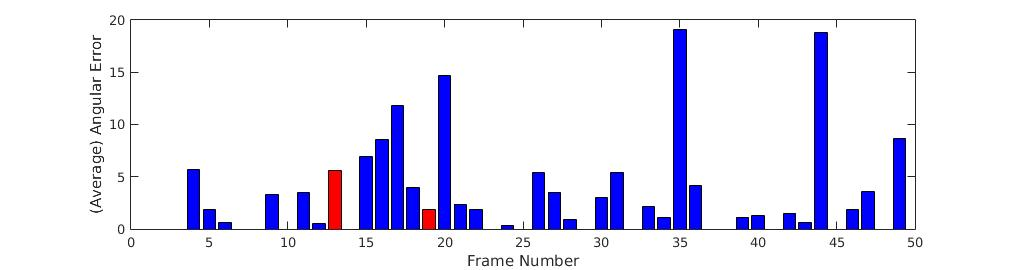
\includegraphics[scale=0.4]{angularerror.jpg}
		\captionsetup{font={small}}
		\caption{ \small (Average) Angular Error versus Frame Number}
		\label{fig:e3}
\end{figure}

\newpage

\subsection{Root Mean Square Error (RMSE)}

Figure \ref{fig:e4} shows the plotted average Root Mean Square Error of each frames.
The RMSE error metric is very sensible to outliers.
But with the outlier removal in the plane cleaning process, a lot of the outliers are removed, this leads to a rather stable distribution of the error values.

Note that some frames with higher RMSE (namely frame 35 and 45). This have lead to a high angular error shown in Figure \ref{fig:e4} above. 
This is not reflected in other frames due to low amount of planes obtained after cleaning plane.
As planes with high errors are usually rejected. 


\vspace{-10pt}
\hspace{-40pt}
\begin{figure}[!h]
		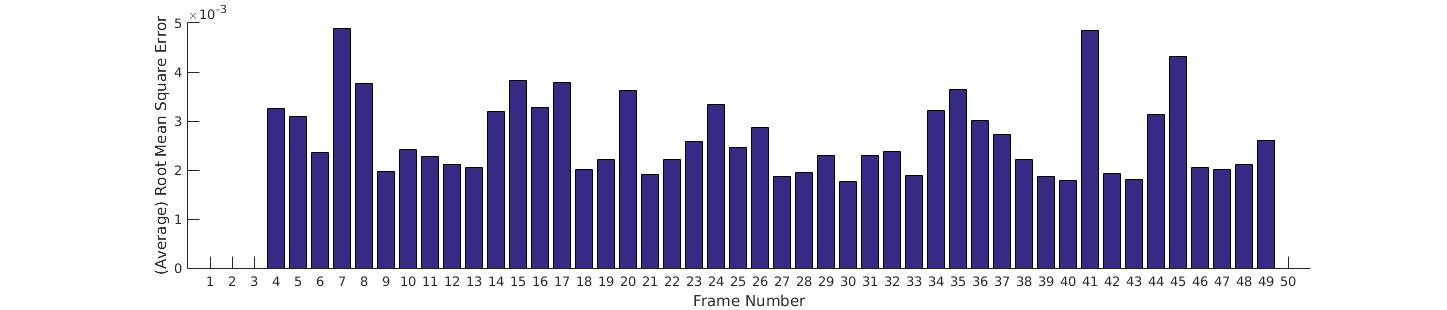
\includegraphics[scale=0.28]{armse.jpg}
		\captionsetup{font={small}}
		\caption{ \small Average Root Mean Square Error of Planes in each image.}
		\label{fig:e4}
\end{figure}

For deeper evaluation of the error, Root Mean Absolute Error (RMAE) is also plotted for the project, where RMAE are sensible to small errors instead of outliers.
However, a similar plot (Figure \ref{fig:e5}) is obtained, this essentially means that most of the outliers are in fact removed. 
Combining with the Angular Error, this high error rate might be caused by the the misfit in the orientation of the planes.

\vspace{-10pt}
\hspace{-40pt}
\begin{figure}[!h]
		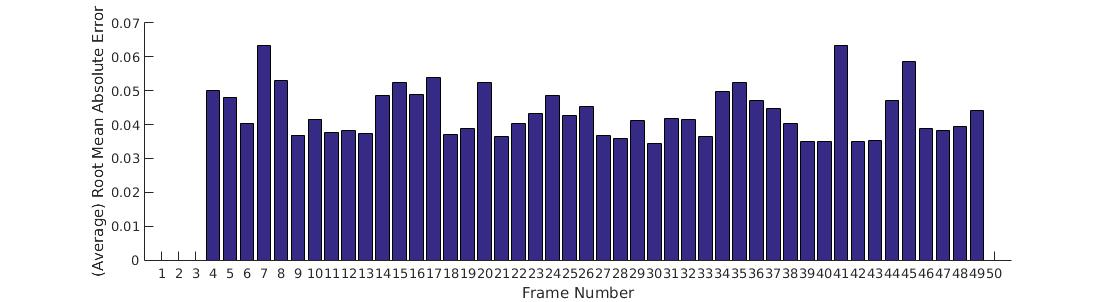
\includegraphics[scale=0.36]{armae.jpg}
		\captionsetup{font={small}}
		\caption{ \small Average Root Mean Absolute Error of Planes in each image.}
		\label{fig:e5}
\end{figure}



\subsection{Overall Performance and Possible Failures}

Overall, the project obtained a relatively clean box with clear surfaces.
However, the time cost of fusing the box is still very time-consuming, which took about 2 minute to form the final model.

One of the reason that leads to the poor speed may be the cleaning plane part. 
Where multiple times of this time-consuming algorithm is performed, in hind-sight this procedure may not be necessary due to the frame could be ignored directly from {\tt model.m} file.
Also, a lot of repetitive operation is used in the project.
The point are repeatedly marked and projected throughout the project.
This also makes the code's structure hard to understand and created a lot of misunderstanding during both coding and creating of the report.

During the mask extraction stage, all the light blue colors are removed. 
If the new box contains such color, it would be removed incorrectly.

Due to the nature of the frame set, not enough plane contains 3 planes.
This could potentially causes the estimation of location of third plane to be wrong in the Rotate Point step in the project.
Also, the handling of this case is not thoroughly tested. 
Fig \ref{fig:e3} shows that there are only 2 frame obtained actually contains 3 useful plane.
This limit of test case could probably make the rotation calculated to be 90 degrees wrong.
However, this error could be fixed with the {\tt model.m} by changing the orientation.

\newpage

\subsection{Table of average RMSE in each frame}

\begin{center}
	\begin{table}[!h]
		\begin{tabular}{|c|c|c|c|}
			\hline
			\makebox[0.2\textwidth][c]{Image name}&\makebox[0.2\textwidth][c]{number of pixels}&\makebox[0.2\textwidth][c]{number of  planes}&\makebox[0.2\textwidth][c]{average RMSE}\\ \hline
			1&$0$&$0$&$N/A$ \\ \hline
			2&$0$&$0$&$N/A$ \\ \hline
			3&$0$&$0$&$N/A$ \\ \hline
			4&$6468$&$2$&$0.00325704261814754$ \\ \hline
			5&$8353$&$2$&$0.00308286767798611$ \\ \hline
			6&$11609$&$2$&$0.00235842065238900$ \\ \hline
			7&$2260$&$1$&$0.00488807060338564$ \\ \hline
			8&$2416$&$1$&$0.00376793312492517$ \\ \hline
			9&$11247$&$2$&$0.00196333671561034$ \\ \hline
			10&$9528$&$1$&$0.00241252775742022$ \\ \hline
			11&$9532$&$2$&$0.00227214416179784$ \\ \hline
			12&$7451$&$2$&$0.00211971044822282$ \\ \hline
			13&$3341$&$3$&$0.00204100727700222$ \\ \hline
			14&$2445$&$1$&$0.00320396658035265$ \\ \hline
			15&$11642$&$2$&$0.00381647358422069$ \\ \hline
			16&$6976$&$2$&$0.00328236431691562$ \\ \hline
			17&$9214$&$2$&$0.00378691254638582$ \\ \hline
			18&$11634$&$2$&$0.00200234314733579$ \\ \hline
			19&$7983$&$3$&$0.00220995176978304$ \\ \hline
			20&$2547$&$2$&$0.00363094831433755$ \\ \hline
			21&$10677$&$2$&$0.00189908399042462$ \\ \hline
			22&$11031$&$2$&$0.00221423739207694$ \\ \hline
			23&$9124$&$1$&$0.00258059149024027$ \\ \hline
			24&$11679$&$2$&$0.00332895449278854$ \\ \hline
			25&$4814$&$1$&$0.00246903180420358$ \\ \hline
			26&$5594$&$2$&$0.00287693104549114$ \\ \hline
			27&$10454$&$2$&$0.00187307024748445$ \\ \hline
			28&$10662$&$2$&$0.00194914242237185$ \\ \hline
			29&$9014$&$1$&$0.00228872457202993$ \\ \hline
			30&$10989$&$2$&$0.00176204488054514$ \\ \hline
			31&$8884$&$2$&$0.00228634363984092$ \\ \hline
			32&$5190$&$1$&$0.00236850564785098$ \\ \hline
			33&$7983$&$2$&$0.00187994303893711$ \\ \hline
			34&$5424$&$2$&$0.00320881566106691$ \\ \hline
			35&$3990$&$2$&$0.00363480957548286$ \\ \hline
			36&$7874$&$2$&$0.00300882760716597$ \\ \hline
			37&$4491$&$1$&$0.00272483638919232$ \\ \hline
			38&$5372$&$1$&$0.00221301979238047$ \\ \hline
			39&$7901$&$2$&$0.00186682583520425$ \\ \hline
			40&$8778$&$2$&$0.00178329528081118$ \\ \hline
			41&$2661$&$1$&$0.00485246559679819$ \\ \hline
			42&$5432$&$2$&$0.00193265584036207$ \\ \hline
			43&$8276$&$2$&$0.00180713930697701$ \\ \hline
			44&$4279$&$2$&$0.00313811247393757$ \\ \hline
			45&$2021$&$1$&$0.00432034233747345$ \\ \hline
			46&$11373$&$2$&$0.00204845955510231$ \\ \hline
			47&$12157$&$2$&$0.00200336568431949$ \\ \hline
			48&$10560$&$1$&$0.00211567933625873$ \\ \hline
			49&$10126$&$2$&$0.00260783666198434$ \\ \hline
			50&$0$&$0$&$N/A$ \\ \hline
		\end{tabular}
		\captionsetup{font={small}}
		\caption{ \small Experimental results}
	\end{table}  
\end{center}



\appendix

\hspace{20pt}

\section{External Code Used}

For plane extraction, the project used the MATLAB functions provided at:

\url{https://www.inf.ed.ac.uk/teaching/courses/av/MATLAB/TASK3/}

Namely, the {\tt getAllPoints} function were used, the {\tt getPlane} function are adapted from the patch growing algorithm.

For transformation linear algebra functions, the following functions are used:
\begin{itemize}
\setlength{\parskip}{-2pt}
\item getPlaneIntersection.m 
\item projectPointOnLine.m
\item getPlaneLineIntersection.m
\item rotx.m 
\item roty.m
\item rotz.m
\end{itemize}

The {\tt rot} functions are from later versions of MATLAB, and the other functions are obtained from:

\url{https://uk.mathworks.com/matlabcentral/fileexchange/17618-plane-intersection}

\url{https://uk.mathworks.com/matlabcentral/fileexchange/17751-straight-line-and-plane-intersection}

\url{https://uk.mathworks.com/matlabcentral/fileexchange/7844-geom2d?focused=8114527&tab=function}


There are also some more efficient distance metric functions (e.g. Euclidean Distance between point/plane) are adapted from various StackOverflow answers. 

\section{References}
Velasquez, H.C. and Fisher, B. 2018. Lab 4.[Online]. School of Informatics, University of Edinburgh. [Accessed 28 March 2018]. Available from:
\url{https://www.inf.ed.ac.uk/teaching/courses/av/DEMOS/lab_4.pdf}\\
\\
Fisher, B. 2018. Advanced Vision Practical. [Online]. School of Informatics. [Accessed 28 March 2018]. Available from: \url{https://www.inf.ed.ac.uk/teaching/courses/av/PRACTICALS/PRACT1/prac11718.pdf}. 


\section{Extract the relevant data from each point cloud}
 \label{algapp:mask} 
\begin{lstlisting}[language=matlab]
%%
function [IMG] = getImage(frameNum, plot)
% Input: frameNum: (int)     The number of frame.
% plot: (boolean) Use of Imshow or not.
% return the image as RGB array.
global pcl_train;

if nargin < 2  
plot = false;
end

img = pcl_train{frameNum}.Color;
IMG = flip(rot90(reshape(img, [512, 424, 3])));

if plot
imshow(IMG);
end

end
%%
function [XYZ] = getDepth(frameNum)
% Input: frameNum: (int)     The number of frame.
% return the xyz locs.
global pcl_train;

img = pcl_train{frameNum}.Location;
XYZ = flip(rot90(reshape(img, [512, 424, 3])));

end
%%
function [mask] = getMask(frameNum)
% Input: frameNum: (int) The number of frame.
% return the mask.
offset = [ 0.15, 0.20, 0.25];
center = [-0.71,-0.30, 0.81];

IMG = getImage(frameNum);
XYZ = getDepth(frameNum);

% BG removal: clears boundary
% Not very useful, table and box have similar color
% BG = double(rgb2gray(getImage(pcl_train,1)));
% mask = abs(double(rgb2gray(IMG))-BG) > 20;

% XYZ boundary
mask = (XYZ(:,:,1) > center(1)-offset(1));
mask(XYZ(:,:,1) > center(1)+offset(1)) = 0;
mask(XYZ(:,:,2) < center(2)-offset(2)) = 0;
mask(XYZ(:,:,2) > center(2)+offset(2)) = 0;
mask(XYZ(:,:,3) < center(3)-offset(3)) = 0;
mask(XYZ(:,:,3) > center(3)+offset(3)) = 0;

%Erode to remove noise
SE1 = strel('square',3);
SE2 = strel('square',4);
mask1 = imerode(imdilate(mask,SE1),SE2);

%Hand HSV
mask2 = removeSkin(IMG);
%Disk because finger?
SE3 = strel('disk',3);
SE4 = strel('disk',7);
mask2 = imdilate(imerode(mask2,SE3),SE4);

%Background Blue
mask3 = removeBlue(IMG);
SE5 = strel('square',10);
mask3 = imerode(imdilate(mask3,SE5),SE5);

%Combine
maskf = bitand(mask1,~mask2);
maskf = bitand(maskf,~mask3);
%Remove points with wrong XYZ
mask = bitand(maskf,mask);
%mask = mask2;
%mask = mask3;
end

%%
function [pc] = getPC(frameNum, filter)
% GETPC Summary of this function goes here
% Detailed explanation goes here

if nargin < 2 
filter = true;
end    

IMG = getImage(frameNum);
XYZ = getDepth(frameNum);
mask = getMask(frameNum);

points={};
rgbs={};

count = 1;
for ii = 1:424
for jj = 1:512
if (~filter) || (mask(ii,jj)~=0)
point = IMG(ii,jj,:);
if ~(point(1)<=0 && point(2)<=0 && point(3)<=0) %?
points{count} = XYZ(ii,jj,:);
rgbs{count} = point;
count = count + 1;
end
end
end
end

pc = pointCloud(cell2mat(points), 'Color', cell2mat(rgbs));
showPointCloud(pc)

end
\end{lstlisting}

\section{Extract the planes from each point cloud}
	\label{algapp:plane} 
\begin{lstlisting}[language=matlab]
%%
function [planes, pts] = getPlanes(xyz, plot)
% GETPLANES return a list of candidate planes
% Input: xyz: a list of coordinate with N x 3 shape.
%        plot: Optional, show the colored planes.
%-----  Set parameter  ----------------------------------------
PLANENUM = 5;     %Max number of planes needed.

PATDISTOL = 0.01;  %Patch-Distance Tolerance.
PATMINPNT = 10;    %Minimum points for a patch to form.
PATMAXRES = 0.0005; %Patch Plane Fitting Error Tolerance. 
PATTRIES = 500;    %Limit attempts to find patches. 

PLANEGROWLIM = 5;   %Limit of times to grow a plane.
PLANEREFITLIM = 50;  %Number of newpoints needed to refit.
PLANEDISTOL = 0.006; %Plane-Distance Tolerance.
PLANEPDISTOL = 2;  %Tolerance between point on same plane.
PLANEMAXRES = 0.005;%Max Average Fitting Error Tolerance 

global SEED; %Random seed for RandPerm
s = RandStream('mt19937ar', 'Seed', SEED);
%---End setting-------------------------------------------------

if nargin < 2 
plot = false;
end

[NPts, W] = size(xyz);
assert(W==3, 'Nx3 shape pls');

planes = zeros(PLANENUM, 4);
remaining = xyz;

if plot
figure(1)
clf
hold on
%plot3(remaining(:,1),remaining(:,2),remaining(:,3),'k.');
end

indexs = 1:NPts;
pts = zeros(NPts,1);

for ii = 1:PLANENUM
%---Init---
fitlist = [];
newlist = [];
fitindex = [];
breaknextfor = false;
%---Patch selection-------------------------------------
L = size(remaining,1); % 8884
idxs = randperm(s,L);
for jj = 1:L
pnt = remaining(idxs(jj),:);
dists = sqrt(sum((remaining-ones(size(remaining))*diag(pnt)).^2,2)); 
mask = dists < PATDISTOL;
if sum(mask) > PATMINPNT %Minimum points for a patch to form.
fitlist = remaining(mask,:);
% Too lazy to optimize this.
[plane,resid] = fitplane(fitlist); 
if resid < PATMAXRES 
remaining = remaining(~mask,:); % update remaining mask
planes(ii,:) = plane;
fitindex = indexs(mask); 
indexs = indexs(~mask);
break
end
end
%Skipped when patch is found.
%When no more patch could be found, skip the next for
%loop to printout result.
if jj == L || jj == PATTRIES
breaknextfor = true;
%disp('no more patches could be found!')
end
end
%---Grow Patch to Plane-----------------------------------
for jj = 1:PLANEGROWLIM
if breaknextfor
breaks
end
distoplane = abs(remaining * planes(ii,1:3)' + planes(ii,4));
% |ax1+bx2+cx3+d|/sqrt(a^2+b^2+c^3+d^2)
mask = distoplane < PLANEDISTOL;
%Is this really necessary? It's very slow.s
%for k = 1:size(mask,1)
%    if ~mask(k)
%        continue
%    end
%    for l = 1:size(fitlist,1)
%        if norm(remaining(k,:)-fitlist(l,:)) < PLANEPDISTOL
%            break;
%        end
%        if l == size(fitlist,1)
%            mask(k) = false;
%        end
%    end
%end
newlist = cat(1,fitlist,remaining(mask,:));

if sum(mask) > PLANEREFITLIM %Number of newpoints needed to refit.
[newplane,fit] = fitplane(newlist);
if fit > PLANEMAXRES * size(newlist,1)
break 
end
planes(ii,:) = newplane;
fitlist = newlist;
remaining = remaining(~mask,:);
fitindex = cat(2,fitindex,indexs(mask));
indexs = indexs(~mask);
continue
end
break %Weird control loop in bob's code.
end
%---End Grow Plane------------------------------------------
pts(fitindex) = ii;
try
if plot
if ii == 1
plot3(newlist(:,1),newlist(:,2),newlist(:,3),'r.');
elseif ii==2 
plot3(newlist(:,1),newlist(:,2),newlist(:,3),'b.');
elseif ii == 3
plot3(newlist(:,1),newlist(:,2),newlist(:,3),'g.');
elseif ii == 4
plot3(newlist(:,1),newlist(:,2),newlist(:,3),'c.'); % Cyan
else
plot3(newlist(:,1),newlist(:,2),newlist(:,3),'m.'); % Magenta
end
end
end
end
end

%%
function [planesout,pointsout] = getCleanPlane(frameNum, plot )
% Input: plot: boolean, optional, self explanatory.
% return a list of planes, and a list of plane allocation.
% set detailed parameters at getPlanes function, dont do it here.
%---Set parameter-----------------------------------------------
MINPNT = 400; %Minimum point needed in plane for it to count.
MAXANG = 15;    %Maximum angle in merge plane phase.
REJANG = 65;   %Minimum angel needed between axis.
ROUND = 5;     %Number of times to run getPlane.m
OUT = 10;       %Maximum number of planes needed.
PLANEDISTOL = 0.01; %Plane-Distance Tolerance.

%---End setting-------------------------------------------------
try
pc = getPC(frameNum);
catch Error
planesout = [];
pointsout = [];
return
end

if nargin < 2 
plot = false;
end

XYZ = squeeze(pc.Location);

planes = [];
points = [];

planesout = [];

%--Get the planes
for i = 1:ROUND
[tempplane, temppoint] = getPlanes(XYZ);
planes = cat(1,planes,tempplane);
points = cat(1,points,histc(temppoint,1:5));
end

%Get most possible plane.
for i = 1:OUT
if numel(points) == 0
break
end
%Sort the remaining
[points, indexs] = sort(points,'descend'); 
if points(1) < MINPNT %Stop if no more good planes
break
end
%Get a list of similar planes
planes = planes(indexs,:);
mask = false(size(points));
mask2 = false(size(points));
u = planes(1,1:3);
for jj = 1:size(points)
if points(jj) < MINPNT
continue
end
v = planes(jj,1:3);
angle = atan2d(norm(cross(u,v)),dot(u,v)); %minimal angle
if angle < MAXANG
mask(jj) = true;
end
if angle < REJANG
mask2(jj) = true;
end
end
%'Average' the candidate planes.
if sum(mask)==1
planesout = cat(1,planesout,planes(mask,:));
else
planesout = cat(1,planesout,mean(planes(mask,:)));
end

%Remove planes have similar angles
points = points(~mask2);
planes = planes(~mask2,:);
end

%prepare output
%Mark all the points 
NPts = size(XYZ,1);
planenum = size(planesout,1);
pointsout = zeros(NPts,1);
index = 1:NPts;
count = 1;
newplaneouts = [];
for i = 1:planenum
%Get distant of everypoint to the plane checking.
distoplane = abs(XYZ * planesout(i,1:3)' + planesout(i,4));
mask = distoplane < PLANEDISTOL; %points in range
%Check size of plane.
mask2 = bitand(mask, pointsout == 0);
if sum(mask2) < MINPNT
continue
end

newplaneouts = cat(1,newplaneouts,planesout(i,:));

mask2 = pointsout > 0; %Currently Marked points
mask2 = bitand(mask, mask2); %Intersect Point
mask = bitand(mask, ~mask2); %Remove the intersection points.

pointsout(index(mask)) = count;
pointsout(index(mask2)) = -1;

%index = index(~mask);
%XYZ = XYZ(~mask,:);
count = count + 1;
end

%Re-mark cross points
for i = 1:size(pointsout,1)
if pointsout(i) == -1
distoplane = abs(XYZ(i,:)*newplaneouts(:,1:3)'+newplaneouts(:,4)');
[~, pointsout(i)] = min(distoplane);
end
end

%plot stuff
if plot
figure(1)
clf
hold on
for i = 1:planenum
mask = pointsout == i;
newlist = XYZ(mask,:);
if i == 1
plot3(newlist(:,1),newlist(:,2),newlist(:,3),'r.');
elseif i==2 
plot3(newlist(:,1),newlist(:,2),newlist(:,3),'b.');
elseif i == 3
plot3(newlist(:,1),newlist(:,2),newlist(:,3),'g.');
end
end

mask3 = pointsout == -1;
mask4 = pointsout == 0;
intersect = XYZ(mask3,:);
XYZ = XYZ(mask4,:);
plot3(intersect(:,1),intersect(:,2),intersect(:,3),'y.');
plot3(XYZ(:,1),XYZ(:,2),XYZ(:,3),'k.');
end
planesout = newplaneouts;
size(planesout,1)
end

\end{lstlisting}

\section{Estimate the 3D positions of the corners where planes meet}
	\label{algapp:corner} 
\begin{lstlisting}[language=matlab]
function [C] = getCorner(arg1, planes, points)
%GETCORNER Summary of this function goes here
%   INPUT: arg1 (frameNum / pc): if frameNum: getPC and other arguments
%if pc: need other argyments
%           planes, points: from getCleanPlane.       
%   OUTPUT: C: if one plane: []
%if two plane: 2x3 matrix of 2 corner points
%if  3  plane: 4x3 matrix of 4 corner points

%---Setting Parameter---
cutoff      = 4;%  For winsor the connect line
cutoffshift = 2;%  Shift % for 3 plane case.
cutoff2     = 3;%  Cutoff % for 3/4th point 
plot = true;
%---Initialize---
%Problematic frames: 7 34 42
C = zeros(3,3);
if nargin < 2
[planes points] = getCleanPlane(arg1);
try
arg1 = getPC(arg1);
catch Error
return
end
end
XYZ = squeeze(arg1.Location);

%--- Ignore if only 1 plane---
NPS = size(planes,1);
if NPS <= 1
C = [];
plot3(XYZ(points==1,1),XYZ(points==1,2),XYZ(points==1,3),'b.');
return
end

% if two lines
if plot
clf;
hold on;
plot3(XYZ(points==1,1),XYZ(points==1,2),XYZ(points==1,3),'b.');
plot3(XYZ(points==2,1),XYZ(points==2,2),XYZ(points==2,3),'g.');
plot3(XYZ(points==3,1),XYZ(points==3,2),XYZ(points==3,3),'r.');
end

mask = bitor(points == 1,points==2);
XYZ2 = XYZ(mask,:);

%Project all points on the connect line.
[P,V,~] = getPlaneIntersection(planes(1,:),planes(2,:));
tps = zeros(size(XYZ2,1),1);
for i = 1:size(XYZ2,1)
[point, tp] = projectPointOnLine(XYZ2(i,:),P,V);
XYZ2(i,:) = point;
tps(i) = tp;
end

%Winsor the line
lower = cutoff; % 4
upper = 100 - lower; % 96
lim = prctile(tps,[lower,upper]); 

%If third plane, shift the winsor direction.
if NPS == 3
[NP,~] = getPlaneLineIntersection(planes(3,:),P,V); 
[~, tp3] = projectPointOnLine(NP,P,V);
if abs(lim(1)-tp3) < abs(lim(2)-tp3)
lower = cutoff - cutoffshift;
upper = 100 - lower;
lim = prctile(tps,[lower,upper]);
else
lower = cutoff + cutoffshift;
upper = 100 - lower;
lim = prctile(tps,[lower,upper]);
end
end

%Remove outlier in the line
mask = bitand(tps>lim(1),tps<lim(2));
XYZ2 = XYZ2(mask,:);
tps2 = tps(mask);
[~, MAX] = max(tps2);
[~, MIN] = min(tps2);
C(1,:) = XYZ2(MAX,:);
C(2,:) = XYZ2(MIN,:);

% In 3-plane's case, points could be shifted.
if NPS == 3
[NP,~] = getPlaneLineIntersection(planes(3,:),P,V);
dists = sqrt(sum((C(1:2,:)-ones(size(C(1:2,:)))*diag(NP)).^2,2));
[~, MAX] = max(dists);
C2 = zeros(4,3);
C2(1,:) = NP;
C2(2,:) = C(MAX,:);
% Also get a third point in plane.
mask = points > 1;
XYZ3 = XYZ(mask,:);
tps = zeros(size(XYZ3,1),1);
for i = 1:size(XYZ3,1)
[point, tp] = projectPointOnLine(XYZ3(i,:),NP,planes(1,1:3));
XYZ3(i,:) = point;
tps(i) = tp;
end
lim = prctile(tps,[cutoff2,100-cutoff2]);
mask = bitand(tps>lim(1),tps<lim(2));
XYZ3=XYZ3(mask,:);
tps=tps(mask);
if mean(tps) < 0
[~, MIN] = min(tps);
C2(3,:) = XYZ3(MIN,:);
XYZ3 = XYZ3(tps < 0,:);
else
[~, MAX] = max(tps);
C2(3,:) = XYZ3(MAX,:);
XYZ3 = XYZ3(tps > 0,:);
end

%And fourth point
mask = bitor(points==1,points==3);
XYZ = XYZ(mask,:);
tps = zeros(size(XYZ,1),1);
crossV = cross(V,planes(1,1:3));
for i = 1:size(XYZ,1)
[point, tp] = projectPointOnLine(XYZ(i,:),NP,crossV);
XYZ(i,:) = point;
tps(i) = tp;
end
lim = prctile(tps,[cutoff2,100-cutoff2]);
mask = bitand(tps>lim(1),tps<lim(2));
XYZ=XYZ(mask,:);
tps=tps(mask);
if mean(tps) < 0
[~, MIN] = min(tps);
C2(4,:) = XYZ(MIN,:);
XYZ = XYZ(tps < 0,:);
else
[~, MAX] = max(tps);
C2(4,:) = XYZ(MAX,:);
XYZ = XYZ(tps > 0,:);
end

%Put C back
C = C2;
if plot
plot3(XYZ3(:,1),XYZ3(:,2),XYZ3(:,3),'b.');
plot3(XYZ(:,1),XYZ(:,2),XYZ(:,3),'g.');
end
end

%Add optional line on 2 plane
if NPS == 2
NP = C(1,:);
mask = points == 2;
XYZ3 = XYZ(mask,:);
tps = zeros(size(XYZ3,1),1);
v = planes(1,1:3);
for i = 1:size(XYZ3,1)
[point, tp] = projectPointOnLine(XYZ3(i,:),NP,v);
XYZ3(i,:) = point;
tps(i) = tp;
end
lim = prctile(tps,[cutoff2,100-cutoff2]);
if mean(tps) < 0
mask = bitand(tps>lim(1),tps<0);
XYZ3=XYZ3(mask,:);
tps=tps(mask);
[~, MIN] = min(tps);
C(3,:) = XYZ3(MIN,:);
else
mask = bitand(tps<lim(2),tps>0);
XYZ3=XYZ3(mask,:);
tps=tps(mask);
[~, MAX] = max(tps);
C(3,:) = XYZ3(MAX,:);
end

mask = points == 1;
XYZ = XYZ(mask,:);
tps = zeros(size(XYZ,1),1);
crossV = cross(V,planes(1,1:3));
for i = 1:size(XYZ,1)
[point, tp] = projectPointOnLine(XYZ(i,:),NP,crossV);
XYZ(i,:) = point;
tps(i) = tp;
end
lim = prctile(tps,[cutoff2,100-cutoff2]);
if mean(tps) < 0
mask = bitand(tps>lim(1),tps<0);
XYZ=XYZ(mask,:);
tps=tps(mask);
[~, MIN] = min(tps);
C(4,:) = XYZ(MIN,:);
else
mask = bitand(tps<lim(2),tps>0);
XYZ=XYZ(mask,:);
tps=tps(mask);
[~, MAX] = max(tps);
C(4,:) = XYZ(MAX,:);
end

if plot
plot3(XYZ3(:,1),XYZ3(:,2),XYZ3(:,3),'b.');
plot3(XYZ(:,1),XYZ(:,2),XYZ(:,3),'g.');
end

end


if plot
plot3(XYZ2(:,1),XYZ2(:,2),XYZ2(:,3),'r.');
scatter3(C(:,1),C(:,2),C(:,3),100,'filled');
hold off;
end

end


\end{lstlisting}

\section{Corners and point clouds normalization} 
	\label{algapp:rotate} 
\begin{lstlisting}[language=matlab]
function [XYZ, C, points] = getRotatedPoints(arg1, C)
%GETROTATEDPOINTS Project the coordinates onto xy,yz,xz planes.
%   arg1 : frameNum/ pc: if not frameNum, use the pc to extract corner.
%                     C: the extracted corner for rotation.
%   output: XYZ: points mapped to plane
%             C: swapped corners
%        points: new marked points (removing points outside the box)


%---Setting Parameter---
removeNegative = true;
plot = true;
%---Initialize---

[planes, points] = getCleanPlane(arg1);
if nargin < 2
try
arg1 = getPC(arg1);
catch Error
return
end
C = getCorner( arg1, planes, points );
end
XYZ = squeeze(arg1.Location);

if size(C,1) == 0
return
end

X = [1 0 0];
Y = [0 1 0];
Z = [0 0 1];

Norm = C(1,:);
C = bsxfun(@minus, C, Norm);
XYZ = bsxfun(@minus, XYZ, Norm);

%Calculate rotation matrix of first axis -- eliminate y;
D = C(2,:);
D(3) = 0;
angle = atan2d(norm(cross(X,D)),dot(X,D));
r = rotz(angle);
D = r * C(2,:)';
if abs(D(2)-0)>0.001
r = rotz(360 - angle);
D = r * C(2,:)';
end

%Calculate rotation matrix of first axis -- eliminate z;
angle = atan2d(norm(cross(X,D)),dot(X,D));
r2 = roty(angle);
D = r2 * (r * C(2,:)');
if abs(D(3)-0)>0.001
r2 = roty(360 - angle);
D = r2 * (r * C(2,:)');
end

%Calculate rotation matrix of second axis
D = r2 * r * C(4,:)';
angle = atan2d(norm(cross(Y,D)),dot(Y,D));
r3 = rotx(angle);
D = r3 * r2 * r * C(4,:)';
if abs(D(3)-0)>0.001
r3 = rotx(360 - angle);
D = r3 * r2 * r * C(4,:)';
end

%Get final rotation matrix.
r = r3 * r2 * r;

%if mismatch, rotate more and swap axis.
%Rotate to negative, (another rotation below rotate it back)
D = r * C(3,:)';
if D(3) > 0
if size(planes,1) == 2
r = roty(180) * r;
D = C(2,:) - C(1,:);
C(2,:) = C(2,:) - 2 * D;
XYZ = bsxfun(@minus, XYZ, D);
end
end

%Put red plane on xy plane, second plane on yz plane.
%For better merging of planes.
%i hate linear algebra.
r = rotz(90) * rotx(180) * r;

for i=1:numel(points)

%Project all points on their plane.
PN = points(i);
if PN == 1
PN = 3;
elseif PN == 2
PN = 4;
elseif PN == 3
PN = 2;
else
%Throw away the urchins
XYZ(i,:) = [0 0 0];
continue
end
point = projectPointOnLine(XYZ(i,:),[0 0 0],C(PN,:));
XYZ(i,:) = XYZ(i,:) - point;
XYZ(i,:) = r * XYZ(i,:)';

end

C = (r * C')';

% Optionally remove all points with negative dim:
if removeNegative
%some error here
mask = sum(XYZ < -0.0002,2) > 0;
points(mask) = 0;
end

% Optionally remove outliers 
% NO, leave the work to C

if plot
clf;
hold on;
xlabel('X')
ylabel('Y')
zlabel('Z')
plot3(XYZ(points==1,1),XYZ(points==1,2),XYZ(points==1,3),'r.');
plot3(XYZ(points==2,1),XYZ(points==2,2),XYZ(points==2,3),'b.');
plot3(XYZ(points==3,1),XYZ(points==3,2),XYZ(points==3,3),'g.');
%plot3(XYZ(points==-1,1),XYZ(points==-1,2),XYZ(points==0,3),'k.');
scatter3(C(:,1),C(:,2),C(:,3),300,'filled');
hold off;
end

end

\end{lstlisting}

\section{Corners and point clouds normalization}
\begin{lstlisting}[language=matlab]
function [pc] = fuseModel()
%COM Summary of this function goes here
%   Detailed explanation goes here

global estimated_size model;

%Optionally remove points outside ze box
removeOutside = true;
%plot = true; %you know you want to plot.

XYZs = [];
RGBs = [];

%Rotation and shifting needed to apply.
%r =  rotx(90);
r = rotx(270) * rotz(180);
norm = - (estimated_size / 2);

for i = 1:50
try
pc = getPC(i);
catch Error
continue
end
[planes,~] = getCleanPlane(i);

[XYZ, ~, points] = getRotatedPoints(i);
IMG = squeeze(pc.Color);

%Compute Normalization and Rotate for Next main plane.
rotate = model(i,1);
if rotate ~= 0

if rotate > 10
rot1 = fix(rotate/10);
rotate = fix(mod(rotate,10));
if rot1 == 1
r = r * rotx(90);
elseif rotate == 3
r = r * rotx(270);
end
end

if rotate == 1
r = r * rotx(90);
elseif rotate == 3
r = r * rotx(270);
elseif rotate == 2
r = r * roty(90);
elseif rotate == 4
r = r * roty(270);
end

end

local_rotate = model(i,2);

if local_rotate >= 1
if local_rotate == 1
r2 = r * rotz(270);
elseif local_rotate == 2
r2 = r * rotz(0);
elseif local_rotate == 3
r2 = r * rotz(90);
else
r2 = r * rotz(180);
end
else
r2 = r;
end

%Normalize the points so the model center at (0,0).
if size(planes,1) <= 1


continue
end

for j=1:numel(points)
XYZ(j,:) = r2 * XYZ(j,:)';

thisnorm = norm .* sign((r2*[1;1;1])');
XYZ(j,:) = XYZ(j,:) + thisnorm;
end

mask = points > 0;
if removeOutside
mask = bitand(mask, XYZ(:,1) < estimated_size(1)/2+0.001);
mask = bitand(mask, XYZ(:,1) >-estimated_size(1)/2-0.001);
mask = bitand(mask, XYZ(:,2) < estimated_size(2)/2+0.001);
mask = bitand(mask, XYZ(:,2) >-estimated_size(2)/2-0.001);
mask = bitand(mask, XYZ(:,3) < estimated_size(3)/2+0.001);
mask = bitand(mask, XYZ(:,3) >-estimated_size(3)/2-0.001);
end

XYZs = cat(1,XYZs,XYZ(mask,:));
RGBs = cat(1,RGBs,IMG(mask,:));
%pc = pointCloud(XYZ(mask,:), 'Color', IMG(mask,:));
pc = pointCloud(XYZs, 'Color', RGBs);
clf;
showPointCloud(pc)
xlabel('X')
ylabel('Y')
zlabel('Z')

pause();
end

end

\end{lstlisting}

\section{Model.m Location Marking File}
\label{app:model}
\begin{lstlisting}[language=matlab]
%Records the details of change to surface, for better merge.

%Random Patches is used to find planes, fix the seed for reproducible
%results. Random seed for RandPerm:

    global SEED estimated_size model;
    SEED = 420;

%Estimated size of the model
%   Use getRotatedPoints function with plot to find this.
%      %Dimension of the X Z Y edge of the box

    estimated_size = [0.17 0.09 0.17];
    %Use the below one for testing
    %estimated_size = [0.9 0.7 0.5];

%Red is main plane, blue is the second (clockwise second if third 
%plane exists) (It may show up as green). 

%Use playPlane2D to estimate this.
 
%below is a matrix showing:
%   first column: Change to red plane
%      0:  not changed
%      1:  changed to top,
%      2:  changed to  right,
%      3:  changed to  bottom,
%      4:  changed to  left,
%      12/14/32/34: Multiple Changes
%   second colum: direction of the "blue" plane.
%      0:  one or less plane is shown,
%      1:  on top,
%      2:  on right,
%      3:  on bottom,
%      4:  on left,

    model = [0 0; ... % 1
             0 0; ... %
             0 0; ... %
             0 1; ... %
             0 1; ... % 5
             0 1; ... % 
             1 0; ... % 
             0 0; ... % 
             1 3; ... % 
             0 0; ... % 10
             0 1; ... % 
             0 1; ... % 
            12 4; ... % 
             4 0; ... % 
             1 3; ... % 15
             0 2; ... % 
             0 1; ... % 
             0 2; ... % 
             2 4; ... % 
             0 2; ... % 20
             2 4; ... % 
             0 4; ... % 
             0 0; ... % 
             0 2; ... % 
             2 0; ... % 25
             0 2; ... % 
             2 4; ... % 
             0 4; ... % 
             0 0; ... % 
             0 2; ... % 30
             2 4; ... % 
             0 0; ... % 
             1 3; ... % 
             0 3; ... % 
             0 2; ... % 35
             0 1; ... % 
             1 0; ... % 
             0 0; ... % 
             0 1; ... % 
             1 3; ... % 40
             0 0; ... % 
             0 1; ... % 
             0 1; ... % 
             1 2; ... % 
             0 0; ... % 45
             2 4; ... % 
             0 4; ... % 
             0 0; ... % 
             0 1; ... % 
             0 0];    % 50
        

\end{lstlisting}

\section{PlayPlane2D: For tracking the location of the planes}
\begin{lstlisting}[language=matlab]
previmage = [];
for i=1:50
    a = getImage(i);
    mask = getMask(i);
    [A,B] = getCleanPlane(i);
    if numel(A) == 0
        %imshow(a);
        pause(0.1);
        continue
    end
    curi = i;
    count = 1;
    for i=1:424
        for j=1:512
            if mask(i,j)
                point = a(i,j,:);
                if ~(point(1)<=0 && point(2)<=0 && point(3)<=0);
                if B(count)==1
                    a(i,j,:) = [255 0 0];
                elseif B(count)==2
                    a(i,j,:) = [0 0 255];
                elseif B(count)==3
                    a(i,j,:) = [0 255 0];
                elseif B(count)==-1
                    a(i,j,:) = [255 255 0];
                end
                count = count + 1;
                end
            end
        end
    end
    if numel(previmage) == 0
        previmage = a;
        continue
    end
    [curi-1 curi]
    a2 = cat(2, previmage, a);
    previmage = a;
    imshow(a2);
    pause();
end
reload;

\end{lstlisting}

\end{document}



%%% Local Variables:
%%% mode: latex
%%% TeX-master: t
%%% End:
